\documentclass[12pt,a4paper]{article}

\usepackage[margin=2.5cm]{geometry}
\usepackage{booktabs}
\usepackage{tabularx}
\usepackage{array}
\usepackage{hyperref}
\usepackage{enumitem}
\usepackage{fancyhdr}
\usepackage{parskip}
\usepackage{titlesec}
\usepackage{xcolor}
\usepackage{graphicx}
\usepackage{float}
\usepackage{mdframed}

\definecolor{accent}{RGB}{30,80,160}
\definecolor{adrbox}{RGB}{240,245,255}

\hypersetup{colorlinks=true, linkcolor=accent, urlcolor=accent}

\titleformat{\section}{\large\bfseries\color{accent}}{}{0em}{}[\titlerule]
\titleformat{\subsection}{\normalsize\bfseries\color{accent}}{}{0em}{}

\pagestyle{fancy}
\fancyhf{}
\lhead{\textbf{WanderSync} \textit{Task 2: Architecture Decision Records}}
\rhead{Team 15}
\rfoot{\thepage}
\renewcommand{\headrulewidth}{0.4pt}

\newcolumntype{L}[1]{>{\raggedright\arraybackslash}p{#1}}

% ADR field command
\newcommand{\adrfield}[2]{%
  \noindent\textbf{#1:}\hspace{0.5em}#2\par\vspace{0.3em}%
}

\begin{document}

\begin{center}
  {\LARGE\bfseries Task 2: Architecture Decision Records}\\[0.4em]
  {\large WanderSync: Dynamic Itinerary, Disruption Management and Social Travel Hub}\\[0.2em]
  {\normalsize Team 15}
\end{center}

\vspace{1em}

% ================================================================
\section{Overview}
% ================================================================

Architecture Decision Records (ADRs) document the significant design decisions made during the
architecture of WanderSync. Each ADR follows the Nygard template, capturing the context that
motivated the decision, the decision itself, and its consequences. The four ADRs below address the
most architecturally significant choices — those whose alternatives were considered and whose
selection has lasting structural implications.

% ================================================================
\section{Architecture Decision Records}
% ================================================================

% ----------------------------------------------------------------
\subsection{ADR-001: Adopt Event-Driven Architecture for Disruption Detection}
% ----------------------------------------------------------------

\begin{mdframed}[backgroundcolor=adrbox, linecolor=accent, linewidth=0.8pt]
\adrfield{Date}{2026-04-20}
\adrfield{Status}{Accepted}
\end{mdframed}

\vspace{0.5em}

\adrfield{Context}{
  Disruption events (flight delays, cancellations, severe weather) originate from external
  third-party feeds that publish updates asynchronously and at unpredictable intervals. A
  synchronous polling model would require the Disruption Detection Service to query each provider
  on a fixed schedule, introducing polling latency, wasted calls during quiet periods, and tight
  temporal coupling between the detection logic and the services that must react to it (Itinerary
  Management, Notification). The core NFR for disruption detection requires at least 85\% accuracy
  across 20 simulated test cases with notification delivery within 10 seconds of event arrival —
  a requirement that favours reactive, push-based processing over synchronous polling.
}

\adrfield{Decision}{
  Adopt an Event-Driven Architecture for the disruption pipeline. The Disruption Detection Service
  subscribes to external feeds via webhooks or short-interval polling and, upon detecting an
  event, persists the event to an internal event log (enabling replay for accuracy auditing) and
  publishes a structured \texttt{DisruptionEvent} message to an internal message broker
  (Redis Pub/Sub or equivalent). The Itinerary Management Service subscribes to this channel,
  updates affected bookings, and delivers user-facing notifications. No direct synchronous call
  exists between the Disruption Detection Service and the Itinerary Management Service.
}

\adrfield{Consequences}{
  \begin{itemize}[noitemsep]
    \item \textit{Positive:} Disruption detection is decoupled from the Itinerary Management
          Service; adding a future consumer (e.g., a dedicated push notification service) requires
          zero changes to the detection service.
    \item \textit{Positive:} Satisfies the 10-second notification delivery requirement; broker
          fan-out is near-instantaneous.
    \item \textit{Positive:} Supports the 85\% accuracy NFR: every \texttt{DisruptionEvent} is
          persisted to an event log before broker publication, enabling deterministic replay
          against the 20 simulated test cases.
    \item \textit{Negative:} Introduces a message broker as a required infrastructure component,
          adding operational complexity and a potential single point of failure (mitigated by
          broker persistence and retry semantics).
    \item \textit{Negative:} Debugging end-to-end flows across async boundaries requires
          structured logging and correlation IDs.
  \end{itemize}
}

\vspace{0.5em}

\textbf{Diagram:} The component diagram below illustrates the event-driven disruption pipeline.
Generate the image from \texttt{diagrams/adr001\_event\_driven.puml} using PlantUML before
compiling the final PDF, then uncomment the figure below.

\begin{figure}[H]
  \centering
  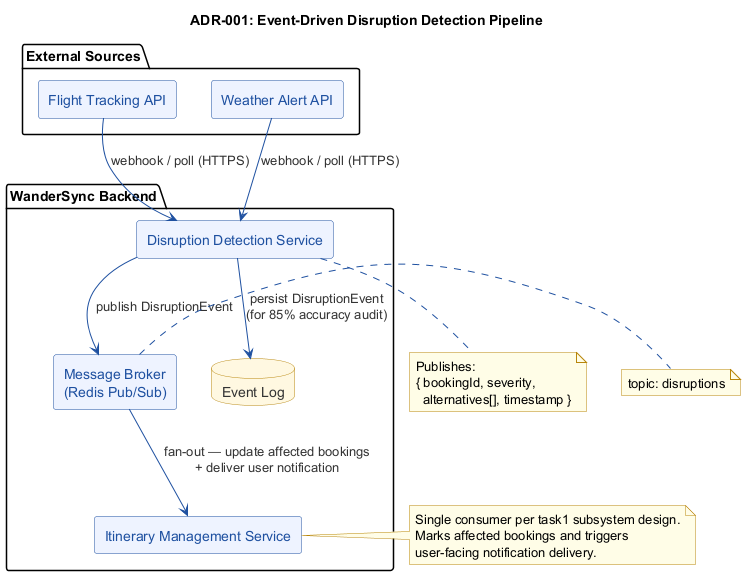
\includegraphics[width=0.85\textwidth]{diagrams/adr001_event_driven.png}
  \caption{ADR-001 — Event-Driven Disruption Detection Pipeline}
\end{figure}

\vspace{1em}

% ----------------------------------------------------------------
\subsection{ADR-002: API Gateway as Single External Entry Point}
% ----------------------------------------------------------------

\begin{mdframed}[backgroundcolor=adrbox, linecolor=accent, linewidth=0.8pt]
\adrfield{Date}{2026-04-20}
\adrfield{Status}{Accepted}
\end{mdframed}

\vspace{0.5em}

\adrfield{Context}{
  WanderSync is composed of multiple independent backend services (Authentication, Booking
  Aggregation, Itinerary Management, Disruption Detection, Social Synchronisation). Without a
  centralised entry point, each service would need to independently manage TLS termination, JWT
  validation, CORS configuration, and rate limiting. This would duplicate cross-cutting security
  logic, create inconsistent enforcement, and expose multiple ports/hostnames to the public
  internet — increasing the attack surface and complicating client-side URL management.
}

\adrfield{Decision}{
  Route all external client traffic through a single API Gateway. The gateway is responsible for:
  TLS termination (HTTPS enforced for all traffic); JWT validation before any request is forwarded
  to a backend service; URL-based routing to the appropriate service; and CORS headers. Backend
  services are not directly reachable by clients and communicate with each other over an internal
  network without TLS overhead.
}

\adrfield{Consequences}{
  \begin{itemize}[noitemsep]
    \item \textit{Positive:} Security policy (JWT enforcement, HTTPS) is centralised and
          consistently applied; no service can be accidentally exposed without auth.
    \item \textit{Positive:} Simplifies client code — one base URL, one auth header convention.
    \item \textit{Positive:} Backend services can be refactored or replaced without changing
          client-facing URLs.
    \item \textit{Negative:} The gateway is a single point of failure for all user-facing traffic;
          requires careful availability management (health checks, restart policy).
    \item \textit{Negative:} All requests traverse the gateway, adding one network hop of latency
          (negligible in local deployment; acceptable for prototype scope).
  \end{itemize}
}

\vspace{0.5em}

\textbf{Diagram:} The deployment diagram below shows the gateway topology. Generate from
\texttt{diagrams/adr002\_api\_gateway.puml}.

\begin{figure}[H]
  \centering
  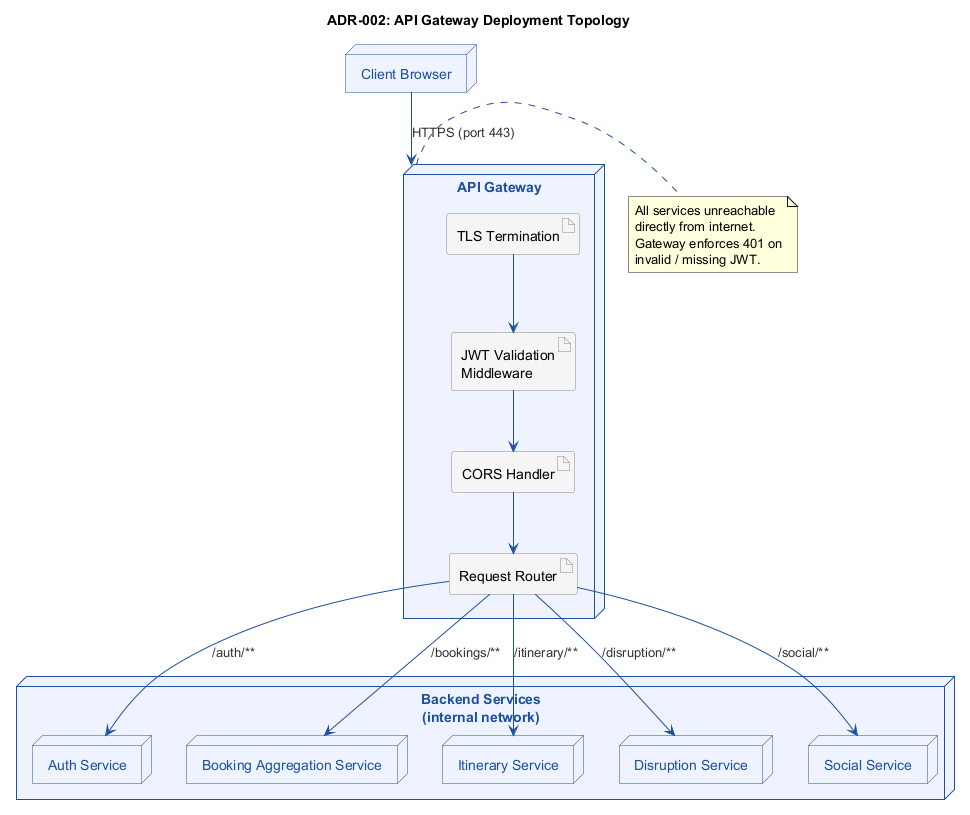
\includegraphics[width=0.85\textwidth]{diagrams/adr002_api_gateway.png}
  \caption{ADR-002 — API Gateway Deployment Topology}
\end{figure}

\vspace{1em}

% ----------------------------------------------------------------
\subsection{ADR-003: Adapter Pattern for Booking Provider Integration}
% ----------------------------------------------------------------

\begin{mdframed}[backgroundcolor=adrbox, linecolor=accent, linewidth=0.8pt]
\adrfield{Date}{2026-04-20}
\adrfield{Status}{Accepted}
\end{mdframed}

\vspace{0.5em}

\adrfield{Context}{
  WanderSync must aggregate booking data from heterogeneous external providers — airlines, hotel
  platforms, and local transport services — each with a distinct API contract and response schema.
  The Modifiability NFR explicitly requires that adding a new travel provider must require changes
  to no more than 2 files outside the dedicated provider adapter module. Without a formal
  structural pattern, direct provider-specific parsing logic would proliferate across the Booking
  Aggregation Service, coupling core business logic to provider-specific details and violating this
  NFR.
}

\adrfield{Decision}{
  Apply the Adapter (Wrapper) design pattern. Define a \texttt{BookingAdapter} interface with a
  single normalisation method \texttt{fetch(userId): List<BookingRecord>}. Each travel provider
  is represented by one concrete adapter class (e.g., \texttt{FlightAdapter},
  \texttt{HotelAdapter}, \texttt{TransportAdapter}) that implements this interface and encapsulates
  all provider-specific API calls and schema mapping. A \texttt{ProviderRegistry} maps provider
  identifiers to adapter instances. Adding a new provider requires: (1) one new adapter file; (2)
  one registration entry in the registry — touching zero other files.
}

\adrfield{Consequences}{
  \begin{itemize}[noitemsep]
    \item \textit{Positive:} Directly satisfies the Modifiability NFR; new providers are additive
          changes with zero impact on core service logic.
    \item \textit{Positive:} The \texttt{BookingAdapter} interface is the only contract that the
          Itinerary Service depends on; providers are interchangeable.
    \item \textit{Positive:} Adapter classes are independently unit-testable with mock provider
          responses.
    \item \textit{Negative:} Requires consistent discipline in keeping all provider logic inside
          adapter classes; code-review enforcement needed to prevent leakage.
    \item \textit{Negative:} The \texttt{BookingRecord} schema must be expressive enough to
          represent all provider data; schema evolution requires careful versioning.
  \end{itemize}
}

\vspace{0.5em}

\textbf{Diagram:} The class diagram below illustrates the Adapter pattern structure. Generate from
\texttt{diagrams/adr003\_adapter.puml}.

\begin{figure}[H]
  \centering
  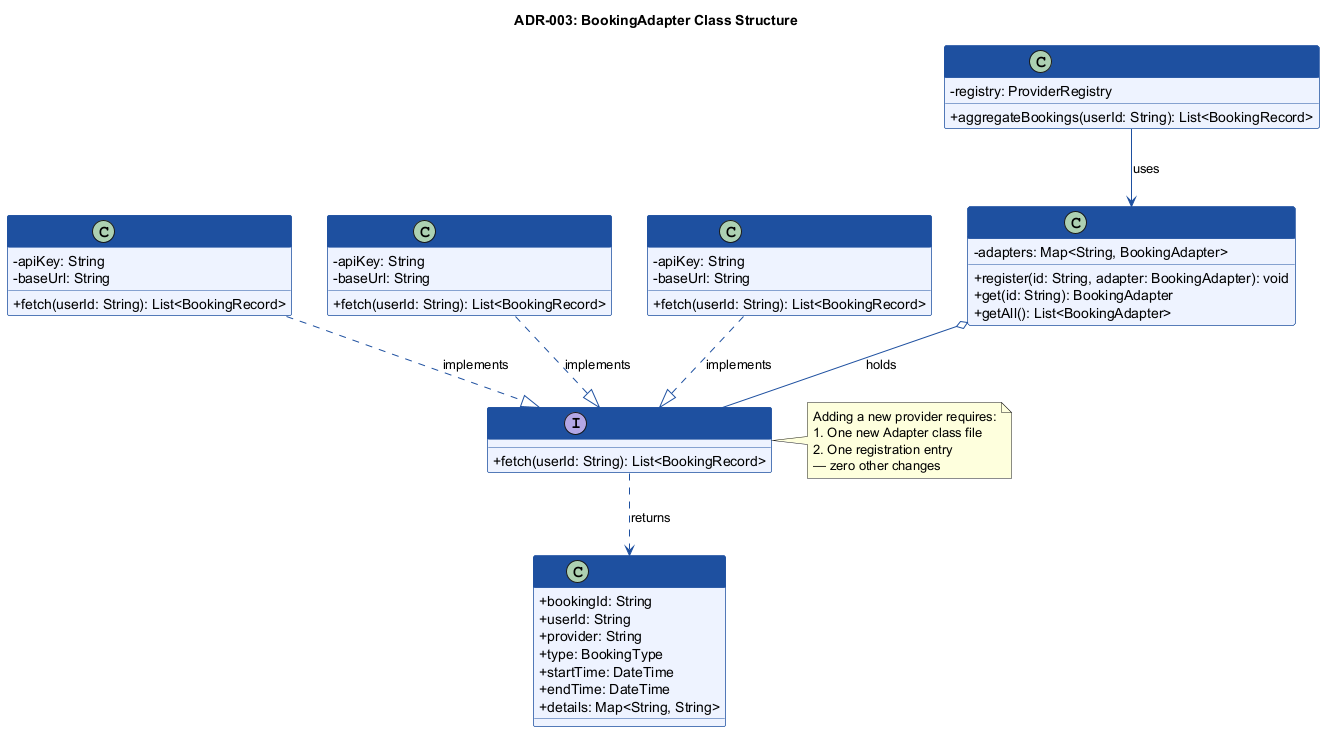
\includegraphics[width=0.85\textwidth]{diagrams/adr003_adapter.png}
  \caption{ADR-003 — BookingAdapter Class Structure}
\end{figure}

\vspace{1em}

% ----------------------------------------------------------------
\subsection{ADR-004: Stateless JWT-Based Authentication}
% ----------------------------------------------------------------

\begin{mdframed}[backgroundcolor=adrbox, linecolor=accent, linewidth=0.8pt]
\adrfield{Date}{2026-04-20}
\adrfield{Status}{Accepted}
\end{mdframed}

\vspace{0.5em}

\adrfield{Context}{
  WanderSync requires that all protected endpoints are inaccessible without a valid user session.
  The two primary authentication models are: (1) \textit{server-side sessions} — the server stores
  session state, each request carries a session ID looked up in a shared store; and (2)
  \textit{stateless tokens} — the server issues a self-contained signed token, each service
  validates it independently with no shared store. With five independent backend services, a
  shared session store would introduce a coupling point and an additional infrastructure dependency.
  The Security NFR specifies JWT tokens with 24-hour expiry and bcrypt password storage.
}

\adrfield{Decision}{
  Adopt stateless JWT-based authentication. The Authentication Service verifies credentials
  (bcrypt hash comparison), issues a signed JWT (HMAC-SHA256, 24-hour expiry) containing the
  user identifier and role claim, and returns it to the client. The client includes the token in
  the \texttt{Authorization: Bearer} header on every request. The API Gateway validates the JWT
  signature and expiry before forwarding; no session store is consulted. Individual backend
  services trust the decoded claims without further auth calls.
}

\adrfield{Consequences}{
  \begin{itemize}[noitemsep]
    \item \textit{Positive:} No shared session store; each service validates tokens independently,
          enabling horizontal scalability and eliminating session-store coupling.
    \item \textit{Positive:} Directly satisfies the Security NFR: bcrypt storage, JWT with
          24-hour expiry, all traffic over HTTPS.
    \item \textit{Positive:} Auth logic is concentrated in the API Gateway middleware; backend
          services are auth-agnostic.
    \item \textit{Negative:} Token revocation before expiry is not supported without a blocklist
          (denylist), which re-introduces state. Accepted as out-of-scope for the prototype;
          24-hour expiry limits the exposure window.
    \item \textit{Negative (Usability — NFR6):} A traveller on a multi-leg journey exceeding
          24 hours will have their session silently expire mid-trip. When the JWT expires, the
          user is prompted to re-authenticate — potentially on unreliable airport Wi-Fi — and will
          be unable to receive disruption notifications until they log in again. A refresh-token
          mechanism or sliding-expiry policy would mitigate this but is deferred to
          post-prototype scope.
    \item \textit{Negative:} Token payload is readable (Base64-encoded); sensitive data must not
          be embedded in claims. Only non-sensitive identifiers (userId, role) are included.
  \end{itemize}
}

\vspace{0.5em}

\textbf{Diagram:} The sequence diagram below shows the JWT issuance and validation flow. Generate
from \texttt{diagrams/adr004\_jwt\_auth.puml}.

\begin{figure}[H]
  \centering
  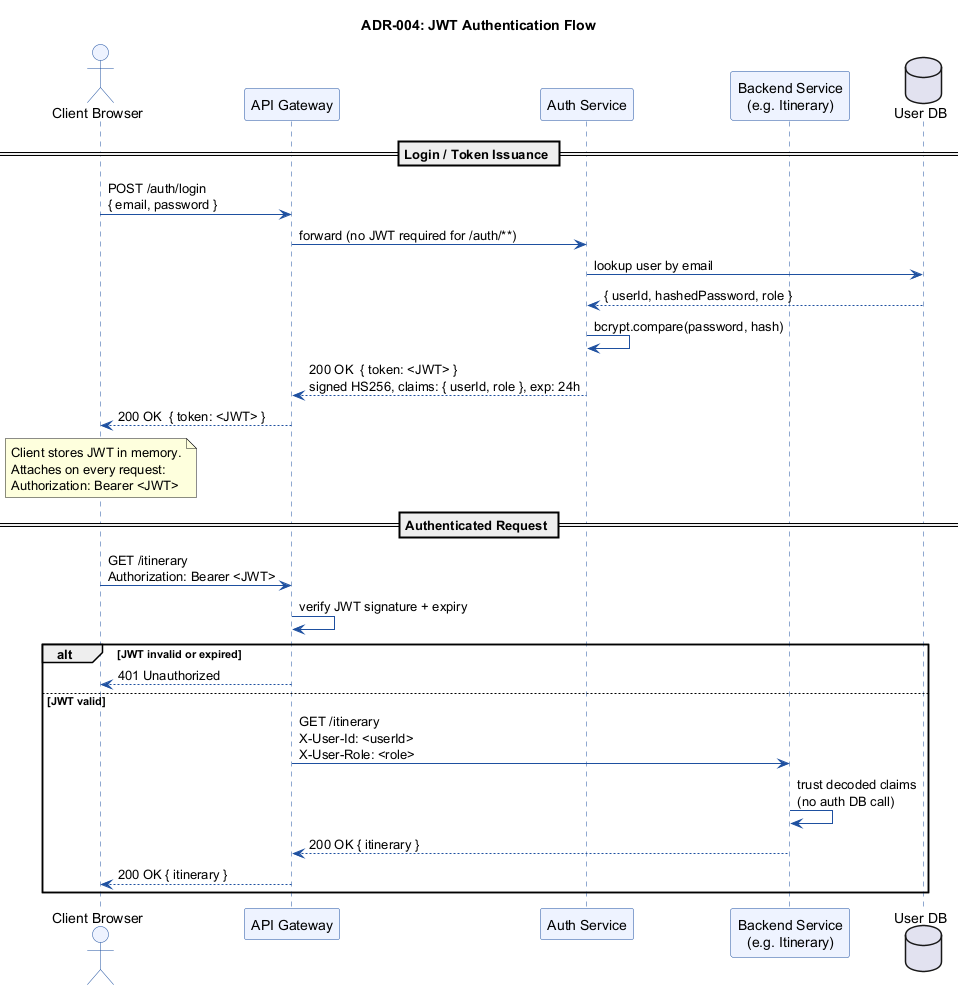
\includegraphics[width=0.85\textwidth]{diagrams/adr004_jwt_auth.png}
  \caption{ADR-004 — JWT Authentication Sequence}
\end{figure}

\end{document}
